\chapter{Background}
\label{chap:Background}


\section{NAND Flash Memory System Software}
In order to overcome the physical limitations of NAND flash memory,
such as the {\it erase-before-write} restriction and the limited P/E cycles,
a special software layer, called a {\it flash translation layer} (FTL), is usually
used in NAND flash memory-based storage systems~\cite{FTL}.
The FTL emulates a normal block device on top of NAND flash memory, thus enabling 
users to use NAND flash memory as if they use block device such as hard disk drives.
The FTL is charge of address mapping, garbage collection, and wear-leveling.
The address mapping function maps a logical block address (LBA) from a host system
to a physical block address (PBA) in NAND flash memory. 
When an update request occurs, the FTL newly allocates a new free page to the request
in NAND flash memory. This update process is called out-place update. 
The location information of the newly allocated page are maintained in the page mapping table
which keeps track of mapping information between LBA and PBA. The old versions of newly written
data remain invalid in the original location. In order to maintain free space in NAND flash memory,
The FTL has to perform a garbage collection process which reclaims the invalid pages in NAND
flash memory. Finally, the wear-leveling procedure induces all blocks in NAND flash memory 
to be evenly erased, thus preventing frequently erased blocks from being repidly worn out
than other blocks.


\section{NAND Flash-Based Storage Devices}
Theoretically, a NAND flash chip with an 8-bit serial bus provides only 40 MB/s for reads
and 13 MB/s for writes. This means that the bandwidth of a single flash chip is seriously 
limited. Moreover, this performance is further reduced with MLC NAND flash memory. 
In order to overcome the limited performance of a single flash chip, flash-based storage 
devices utilize the parallelism of multiple NAND flash chips.

\begin{figure*}[b]
	\centering
	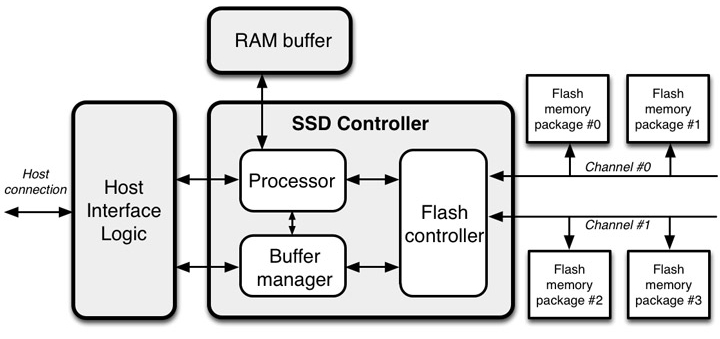
\includegraphics[width=0.8\textwidth]{figure/background/ssd_arch}
	\caption{A simplified diagram of typical SSD.}
	\label{fig:ssd_arch}
\end{figure*}

Figure~\ref{fig:ssd_arch} shows a simplified diagram of typical NAND flash-based storage
devices, consisting of a processor, flash controller, several flash memory packages, and
host interface logic. The FTL running on the processor receives host commands (e.g., reads
and writes) through the host interface module from the host system, and then issues several
flash I/O commands to the flash controller. The flash controller handles multiple I/O commands
simultaneously. Thus, it is possible to achieve much higher performance than utilizing
a single NAND flash chip, providing the aggregate bandwidth of multiple flash chips
with the host system.

\section{Multi-stream Interface}
At the heart of the garbage collection problems of SSD are the issues of
how to predict the lifetime of data written to the SSD and
how to ensure that data with similar lifetime are placed in
the same erase unit. Kang et. al.~\cite{MultiStream}, proposed multi-streaming,
an interface that directly guides data placement within
the SSD, separating the two issues. Authors argue that the
host system should (and can) provide adequate information
about data lifetime to the SSD. It is the responsibility
of the SSD, then, to place data with similar lifetime (as
dictated by the host system) into the same erase unit.

The design introduces the concept of stream. A stream
is an abstraction of SSD capacity allocation that stores a
set of data with the same lifetime expectancy. An SSD
that implements the proposed multi-stream interface allows
the host system to open or close streams and write to
one of them. Before writing data, the host system opens
streams (through special SSD commands) as needed.
Both the host system and the SSD share a unique stream
ID for each open stream, and the host system augments
each write with a proper stream ID. A multi-streamed
SSD allocates physical capacity carefully, to place data
in a stream together and not to mix data from different
streams.


Figure~\ref{fig:multistream} shows the example of block allocation with and without
multi-stream. Without Multi-stream, data are written in the order in which 
they are received. As a result, different lifetimes of data are mixed in the same block.
It incurs high valid page copy overhead for garbage collection due to the different 
invalidation time.
However, with Multi-stream, data with same lifetime are separated in a different block
so that they are likely to be invalidated together that results low garbage collection overhead.
In order to maximize the effect of the multi-streamed SSD, identifying similar lifetime data
is the most important and difficult.

\begin{figure*}[t]
	\centering
	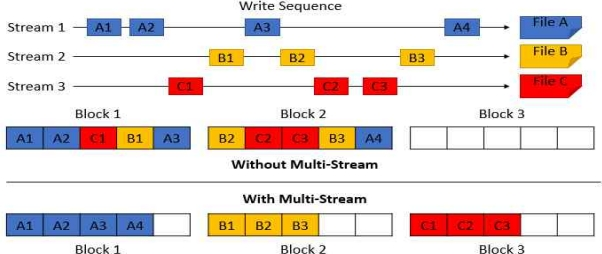
\includegraphics[width=0.8\textwidth]{figure/background/multistream}
	\caption{Block allocation with and without multi-stream.}
	\label{fig:multistream}
\end{figure*}


\section{Inline Data Deduplication Technique}
Inline deduplication saves the lifetime of SSDs more than
offline deduplication~\cite{InlineDedup}. The lifetime of SSD flash cells is limited to a
specified small number of writes and block erasures (e.g., around
5,000 times in MLC SSD). Inline deduplication minimizes the number
of writes to the SSDs by writing only unique data blocks. However,
offline deduplication requires writing all duplicate and unique blocks
to the SSDs first. Then during the idle time, stored data are read, and
the unique ones are written back to respective SSDs.

Inline data deduplication typically consists of four steps. First, the
deduplication module receives a write request with data ($Data_a$)
and logical block address ($LBA_a$). Second, $Data_a$ are chunked into
fixed-sized blocks or variable-sized blocks. In this dissertation, we use
fixed-sized chunking which has a lower CPU utilization requirement
and has been commercially used in primary storage~\cite{InlineDedup}.
Third, the module calculates a signature ($Sig_a$) for the data. Fourth,
the module looks up $Sig_a$ in the deduplication tables. If the
signature matches another signature ($Sig_b$) that was already stored
in the deduplication tables, the received write request is considered
duplicate ($Data_a = Data_b$). Then Dataa will not be written to the
storage devices and the module only updates the deduplication
tables. The update includes recording a mapping from $LBA_a$ to the
physical block address ($PBA_b$) of the matched signature. For cases
that step four cannot find $Sig_a$ in the table, the write request is considered
unique. Therefore, in addition to updating the deduplication
tables, $Data_a$ are written to the storage devices.
%A Scalable HW-Based Inline Deduplication for SSD Arrays

\section{Related Work} 
\subsection{Data Separation Techniques for Multi-streamed SSDs}
There are several research for detecting data temperature. Park, et al.~\cite{multibloom} 
uses multiple bloom
filters to identify hot data in the device layer. Stoica, et al.~\cite{updatefreq}
propose new data placement algorithms to improves
flash write performance by estimating data update frequencies.
Luo, et al.~\cite{writehot} observe high temporal write
locality in different workloads and design a write-hotness
aware retention management policy to improve flash memory
life time. Most research is on a simulation or mathematical
modeling basis and those lack of real world system and
performance analysis. It is hard to guarantee the benefit
of these algorithms in a dynamic I/O intensive datacenter
workloads. In adition, as multi-stream SSDs
become available, there is a need to identify data temperature
and separate them to multiple levels (usually more
than three levels - hot, cold and warm) to fully utilize such
devices.

There have been many studies for multi-streamed SSDs ~\cite{MultiStream, Level,
vStream, FStream, AutoStream, PCStream}.  Kang {\it et al.} first proposed a
multi-streamed SSD that supported manual stream allocation for separating
different types of data~\cite{MultiStream}.  Yang {\it et al.} showed that a
multi-streamed SSD was effective for separating data of append-only
applications like RocksDB~\cite{Level}.  Yong {\it et al.} presented a virtual
stream management technique that allows logical streams, not physical streams,
to be allocated by applications.  Unlike these studies that involve modifying
the source code of target programs, \textsf{\small PCStream} automates the
stream allocation with no manual code modification.

Rho {\it et al.} proposed a stream management technique, called FStream, at the
file system layer~\cite{FStream}. In FStream, metadata, journal
data, and user data that may have different lifetime characteristics were
allocated to separate streams.  Since FStream was implemented as a part of a file
system, it was not able to directly detect application's I/O behaviors.
Also, it may be hard to be deployed in practice due to 
a strong dependence on file system-specific implementation details.
\textsf{\small PCStream}, on the other hand, efficiently exploits
programs' I/O behaviors using PCs with no file system-specific modifications.

Yang {\it et al.} presented an automatic stream management technique at the
block device layer~\cite{AutoStream}. Similar to hot-cold data separation
technique used in FTLs, it approximates the data lifetime of data based on
update frequencies of LBAs.  The applicability of this technique is, however,
quite limited to in-place update workloads only.  \textsf{\small PCStream} has
no such limitation on the workload characteristics, thus effectively working
for general I/O workloads including append-only, write-once 
as well as in-place update workloads.

Ha {\it et al.} proposed an idea of using PCs to separate hot data from cold
one in an FTL layer~\cite{PCHa}.  Kim {\it et al.} extended it for
multi-streamed SSDs~\cite{PCStream}.  Unlike these work, our study treats the
PC-based stream management problem in a more complete fashion by (1)
pinpointing the key weaknesses of existing multi-streamed SSD solutions, (2)
extending the effectiveness of PCs for more general I/O workloads including
write-once patterns, and (3) introducing internal streams as an effective
solution for outlier PCs.  Furthermore, \textsf{\small PCStream} exploits the
globally unique nature of a PC signature for supporting short-lived
applications that runs frequently.



\subsection{Write Traffic Reduction Techniques}
In order to extend the lifetime of flash-based SSDs,
data deduplication techniques have been used in recent SSDs
because they are effective in reducing the amount of data written to flash memory by preventing duplicate data from being written again~\cite{caftl,value-locality}.
As a result, only non-duplicate data, i.e., unique data, are stored in SSDs effectively decreasing the total amount of data written to
SSDs.
In most deduplication schemes proposed for SSDs,
the unit of data deduplication is same as the flash page size which is usually 4 KB or 8 KB.
Using a page as a deduplication unit seems to be reasonable 
because the unit of a read or write operation of flash memory is also a page. 
However, this page-based deduplication technique misses many chances of eliminating duplicate data, especially
when two pages are \textit{almost} identical.
For example, in our experimental analysis of an existing 4 KB page-based deduplication technique, we observed that
up to 34\% mostly identical data.
If the unit of deduplication were smaller than 4 KB, about 23\% more data could be identified as duplicate data.
%We observed that up to 48\% of unique pages actually contain mostly identical data.
%The existing techniques, however, can not completely eliminate the duplicate segment in those pages 
%since they are considered as unique pages.
Furthermore, it is expected that the effectiveness of the page-based deduplication technique would 
get even worse in future NAND flash memory as the page size of 
flash memory is expected to increase
to a bigger size such as 16 KB~\cite{16kpage}.

%In our observation, many pages are rewritten to flash memory after being modified slightly.
%Thus, the contents of the previous page and the new one are nearly identical.
%{\color{red}In our observation, however,
%this page-based deduplication loses many chances of eliminating duplicate data because of following two reasons.
%( ).}

%In order to extend the limited lifespan, data deduplication technique, which removes redundant data from the workload,
%has been widely adopted in SSDs. 
%In the existing scheme, the size of a chunk, which is used as a unit of redundancy checking and writing, is commonly 
%fixed to the page size of the flash memory to minimize the additional management overhead.
%Using page-sized chunking method, however, slightly modified data chunk can not be determined as duplicated data although
%most of data in the chunk are the same, i.e. \textit{partially matched data}.
%Furthermore, the portion of \textit{partially matched data} is expected to be even significantly larger when the flash page size 
%becomes bigger as the semiconductor technology scales down.
%For example, the page size of initial SLC flash memory was 2KB.%~\cite{2kpage}. 
%The 4KB-sized page has become more common in both industry and research in the late 2000s.%~\cite{4kpage1,4kpage2,4kpage3}. 
%In the early 2010s, the scaling trend has been accelerated so 
%that the flash page size has become 8KB%~\cite{8kpage1,8kpage2} 
%and even 16KB. %~\cite{16kpage}. 
%Under the \textit{large-page} flash memory, the existing deduplication techniques
%for SSDs have unavoidable limitations since the probability of finding pages with an exact match will be significantly low.
%---------------------------------------------

%The most well-known approach that improves the storage lifetime is to optimize flash firmware algorithms. 
%As mentioned previously, 
Because of the ``erase-before-write'' nature of NAND flash memory, 
flash storage devices employ a flash translation layer (FTL) 
that supports address mapping, garbage collection, and wear-leveling algorithms~\cite{FAST}. %~\cite{BAST,FAST,LAST}.
These firmware algorithms incur a lot of extra write/erase operations,
seriously shortening the overall lifetime of a storage device.
For this reason, a large number of studies have been focused on reducing such extra operations to improve the storage 
lifetime.
%The firmware-level optimization has been effective in improving the lifetime of flash-based SSDs. 
However, considering the decreasing lifetime of recent high-density NAND flash memory such as TLC NAND flash memory~\cite{tlc}, %~\cite{mlc1,mlc2}, 
more aggressive lifetime management solutions are required. 

Data deduplication techniques, which are originally developed for backup systems,
are regarded as one of the promising approaches for extending the storage lifetime
because of their ability that reduces the amount of write traffic sent to a storage device.
In deduplication techniques, a chunk is used as an unit of identification and elimination of duplicate data.
%An unit of verification of duplicate and elimination is called chunk in deduplication techniques.
Depending on their chunking strategies, deduplication techniques can be categorized into two types,
fixed-size deduplication and variable-size deduplication.
Fixed-size deduplication divides an input data stream into fixed-size chunks (e.g., pages)~\cite{caftl,value-locality}. %~\cite{caftl,value-locality,idedup}.
Then, it decides if each chunk data is duplicate and prevents duplicate chunks %whose data are already stored in flash memory 
from being rewritten to flash memory.
Unlike fixed-size deduplication, 
the chunk size of variable-size deduplication is not fixed.
Instead, it decides a cut point between chunks using 
a content-defined chunking (CDC) algorithm
which divides the data stream according to the contents~\cite{dedupv1, dong}.

% SSD의 경우 fixed-size dedup을 할 수 밖에 없음을 강조
In general, variable-size deduplication techniques can identify more data as duplicate data than the fixed-size deduplication technique.
Since variable-size deduplication adaptively changes the size of chunks by analyzing the contents of input stream,
duplicate data are more effectively found regardless of their locations.
In spite of its advantages, variable-size deduplication is not commonly used in SSDs because of the following practical limitations.

First, the CDC algorithm often requires relatively high computational power and a large amount of memory space. 
Thus, variable-size deduplication is not appropriate to be employed at the level of 
storage devices where computing and memory resources are constrained. 
Second, the size of remaining unique data after deduplication may vary in variable-size deduplication. 
When writing those data, a complicated scheme for data size management is required 
to form sub-page data chunks to fit in a flash page size, preventing an internal fragmentation. 
For those reasons, most existing deduplication techniques for SSDs employ fixed-size deduplication, 
which is relatively simple and does not require a significant amount of hardware resources.

There are several existing studies for fixed-size deduplication for SSDs. F. Chen~\cite{caftl} proposed CAFTL 
to enhance the endurance of SSDs with a set of acceleration techniques to reduce runtime overhead. 
A. Gupta~\cite{value-locality} also proposed CA-SSD to improve the reliability of SSDs by exploiting the value locality, 
which implies that certain data items are likely to be accessed preferentially. 
In these studies, authors focused on the feasibility of deduplication at SSD level and 
proved its effectiveness rather than improving deduplication itself.

Recently, several deduplication techniques for flash-based storage are proposed. Z. Chen~\cite{order-merge}
proposed OrderMergeDedup which orders and merges the deduplication metadata with data writes to 
realize failure-consistent storage with deduplication.  
W. Li~\cite{cachededup} proposed CacheDedup which integrates deduplication with caching architecture to 
address limited endurance of flash caching by managing data writes and deduplication metadata together, 
and proposing duplication-aware cache replacement algorithms. 
These studies focus on systematic approach such as block layer or flash caching. 
However, this study improves the effect of deduplication in the device-specific domain, 
so the approach of this study is quite different.

Similar to the existing deduplication techniques,
the proposed FineDedup technique is also based on fixed-size deduplication.
Using a smaller deduplication unit,
however, FineDedup improves the likelihood of eliminating duplicate data.
This approach can complement the limitation of existing fixed-size deduplication techniques,
which exhibit a relatively low amount of removed writes 
in comparison with variable-size deduplication.

\subsection{Program Context based Optimization Techniques for Operating Systems}
History-based prediction techniques exploit the principle
that most programs exhibit certain degrees of repetitive
behavior. For example, subroutines in an application are
ckalled multiple times, and loops are written to process a
large amount of data. The challenge in making an accurate
prediction is to link the past behavior (event) to
its future reoccurrence. In particular, predictors need the
program context of past events so that future events about
to occur in the same context can be identified. The more
accurate context information the predictor has about the
past and future events, the more accurate prediction it can
make about future program behavior.

A key observation made in computer architecture is that
a particular instruction usually performs a very unique
task and seldom changes behavior, and thus program instructions
provide a highly effective means of recording
the context of program behavior. Since the instructions
are uniquely described by their program counters (PCs)
which specify the location of the instructions in memory,
PCs offer a convenient way of recording the program context.

One of the earliest predictors to take advantage of the
information provided by PCs is branch prediction. 
The PC of the branch instruction uniquely identifies
the branch in the program and is associated with a particular
behavior, for example, to take or not to take the
branch. Branch prediction techniques correlate the past
behavior of a branch instruction and predict its future behavior
upon encountering the same instruction.

The success in using the program counter in branch
prediction was noticed and the PC information has been
widely used in other predictor designs in computer architecture.
Numerous PC-based predictors have been
proposed to optimize energy~\cite{cacheenergy}, cache management~\cite{cachemngmt}
, and memory prefetching~\cite{memoryprefetching}. 
For example, PCs have been used to accurately predict
the instruction behavior in the processor's pipeline
which allows the hardware to apply power reduction techniques
at the right time to minimize the impact on performance~\cite{cacheenergy}
. In Last Touch Predictor~\cite{cachemngmt}, PCs are
used to predict which data will not be used by the processor
again and free up the cache for storing or prefetching
more relevant data. In PC-based prefetch predictors~\cite{memoryprefetching}
, a set of memory addresses or
patterns are linked to a particular PC and the next set of
data is prefetched when that PC is encountered again.

Moreover, PCC~\cite{PC} considers the opportunity and 
viability of PC-based prediction techniques
in operating systems design. In particular, they consider
the buffer cache management problem, which shares common
characteristics with hardware cache management as
they essentially deal with different levels of the memory
hierarchy.
The basic idea is to separate access streams by the program
context (identified by the function call stack) when the I/O
access is made, with the assumption that a single program
context is likely to access disk files with the same pattern in
the future.

However, none of the existing PC-based approach focus of the storage devices.
They use iterative access characteristics according to the PC 
at the operating system level, e.g., cache management.
Based on our analysis on PCs, program context can be a good candidate 
for optimizing performance and lifetime of SSDs.
